\subsubsection{Pods}
\label{subsec:kubernetes:pods}
Ein Pod repräsentiert eine Sammlung von laufenden Anwendungscontainern 
und Volumes (siehe \ref{subsec:kubernetes:volume}) in der selben Umgebung.
Hierbei sind Pods die kleinste Einheit innerhalb eines Kubernetes Clusters, wodurch alle Container eines Pods
immer auf dem selben Knoten betrieben werden \cite{Burns2019}.
Alle Container innerhalb eines Pods teilen sich Netzwerkschnittstellen, Speicher und Hardwareresourcen \cite{kubernetesPods},
sind jedoch von anderen Pods isoliert \cite{Burns2019}.

\begin{figure}[h]
  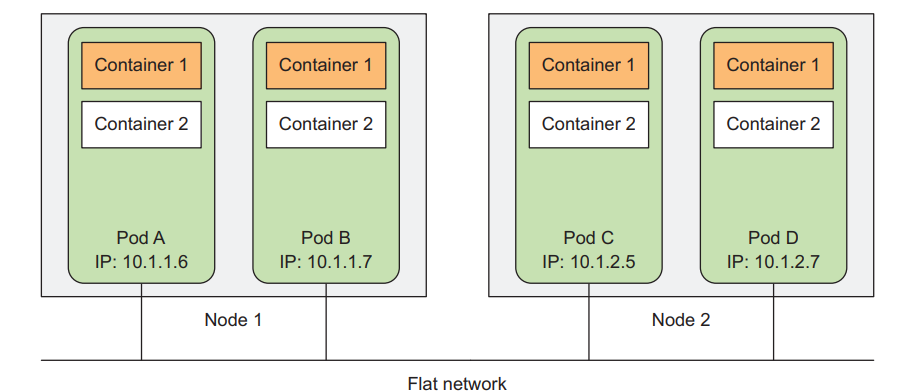
\includegraphics[width=\textwidth]{gfx/chapters/2_grundlagen/kubernetes_network.png}
  \caption{Beispiel zur Provisionierung der Pods innerhalb des Clusters}
  \label{fig:kubernetes_network}
  \source{\cite{Marko2018}}
\end{figure}

In \ref{fig:kubernetes_network} wird dargestellt, wie Pods innerhalb eines Cluster betrieben werden.
Jeder Pod im Kubernetes Cluster befindet sich in einem großen Netzwerk, in dem Pods mittels IP-Addressen untereinander 
kommunizieren können \cite{Marko2018}. 


